\subsection{Data Extraction in PRISM}

The data used in this study originate from PRISM, a platform created by AEPW that integrates plastic waste, demographic, and socioeconomic data from various public sources into a usable format.

\begin{figure}[H]
	\centering
	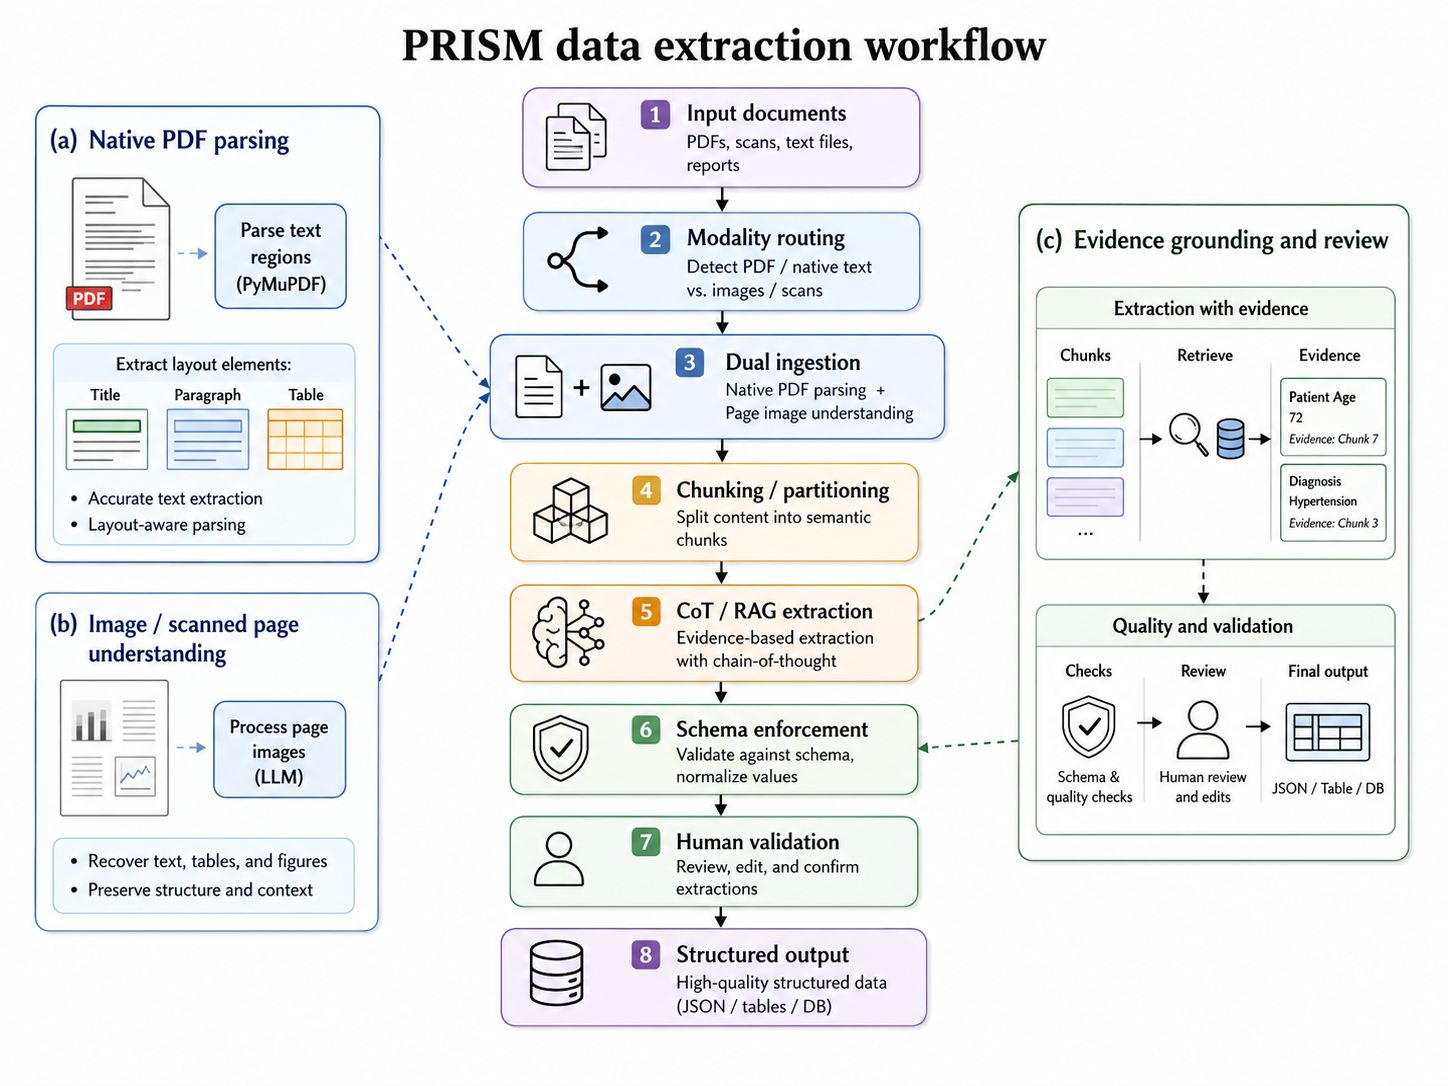
\includegraphics[width=1.0\linewidth]{figures/prism_data_extraction.png}
	\caption{
		PRISM data extraction workflow.
		The system first identifies the input document type, either a PDF or a tabular file.
		For PDF documents, PRISM uses \texttt{PyMuPDF} to parse text regions and extract layout elements, while images are processed to recover text, tables, and figures using large language models (LLMs).
		Parsed content is then chunked, indexed, and processed through evidence-grounded extraction using LLMs.
		Subsequently, the extracted data undergo schema enforcement and human validation before being used in downstream analysis.
	}
	\label{fig}
\end{figure}

Figure~\ref{fig} illustrates the data extraction workflow used by the PRISM platform to transform unstructured documents such as PDF and Excel files into structured data.
Two different parsers are applied depending on the type of input document.
Layout elements such as images, charts, and tables are interpreted using GPT-4o to generate meaningful contextual information.
PDF files are parsed using the \texttt{PyMuPDF} library, whereas Excel files are read using the \texttt{pandas} library.

After parsing, the PDF pipeline stores embedded text chunks in Azure AI Search to support retrieval-augmented generation for selected fields such as publisher and report date.
Large language models are then applied to identify relevant data points, including year, location, data point name, value, unit, and source context.
Retrieval-Augmented Generation (RAG) is used to extract publisher names and report dates, while Chain-of-Thought (CoT) prompting is applied to extract data points from Excel files.
Subsequently, the extracted outputs are passed through multiple post-processing layers, including data cleaning, location and data point mapping, duplicate removal, unit standardization, calculated field generation, and quality score computation.
Finally, the structured extraction results are appended to the database.

Because automated extraction using LLMs can produce inaccurate results, PRISM employs a human validation workflow.
Extracted records are initially marked as unvalidated and can be approved or rejected by authorized reviewers.
The platform records the validation status and associated validation metadata before approved records are made available for downstream use.
The available PRISM documentation does not identify the number or qualifications of the reviewers who validated the records used in this study.
